\documentclass[a4paper,12pt]{article}
\usepackage{amssymb} %\mathbb
\usepackage{amsmath} % {align}
\usepackage{xcolor}
\usepackage{verbatim}
\usepackage{listings}
\usepackage{multirow}
\usepackage{graphicx}
\usepackage{hyperref}
\hypersetup{
    colorlinks=true,
    linkcolor=blue,
    filecolor=magenta,      
    urlcolor=cyan,
    pdftitle={ECE655\_Project\_2},
    pdfpagemode=FullScreen,
    }
\usepackage{subcaption}
\usepackage{wrapfig}
%\usepackage[most]{tcolorbox}
\usepackage[utf8]{inputenc}
\usepackage[english]{babel}
\usepackage{booktabs}
\usepackage{mdframed}
\usepackage{makecell}
\usepackage{array}
\usepackage{pbox}
\usepackage{textcomp}
\usepackage{upgreek}
\usepackage{gensymb}
\usepackage{longtable}
\usepackage{enumerate}
\usepackage{enumitem}
\usepackage{booktabs} % To thicken table lines
\usepackage{hyphenat}
\usepackage{url}
\usepackage{hyperref}

\definecolor{codegreen}{rgb}{0,0.6,0}
\definecolor{codegray}{rgb}{0.5,0.5,0.5}
\definecolor{codepurple}{rgb}{0.58,0,0.82}
\definecolor{backcolour}{rgb}{0.95,0.95,0.92}
\definecolor{filename}{rgb}{0.1,0.1,0.99}
\definecolor{textout}{rgb}{0.3,0.4,0.3}

\newcommand{\purple}[1]{\textsf{\textcolor{codepurple}{#1}}}

\lstdefinestyle{mystyle}{
    backgroundcolor=\color{backcolour},   
    commentstyle=\color{codegreen},
    keywordstyle=\color{magenta},
    numberstyle=\tiny\color{codegray},
    stringstyle=\color{codepurple},
    basicstyle=\ttfamily\footnotesize,
    breakatwhitespace=false,         
    breaklines=true,                 
    captionpos=b,                    
    keepspaces=true,                 
    numbers=left,                    
    numbersep=5pt,                  
    showspaces=false,                
    showstringspaces=false,
    showtabs=false,                  
    tabsize=2
}

\lstset{style=mystyle}

%\renewcommand{\texttt}[1]{%
%  \begingroup
%   \ttfamily
%   \begingroup\lccode`~=`/\lowercase{\endgroup\def~}{/\discretionary{}{}{}}%
%   \begingroup\lccode`~=`[\lowercase{\endgroup\def~}{[\discretionary{}{}{}}%
%   \begingroup\lccode`~=`.\lowercase{\endgroup\def~}{.\discretionary{}{}{}}%
%   \catcode`/=\active\catcode`[=\active\catcode`.=\active
%   \scantokens{#1\noexpand}%
%   \endgroup
% }

% Define todo                                                                   
\newcommand{\TODO}[1]{\textcolor{red}{[TODO: #1]}}
\newcommand{\ans}[1]{\textcolor{blue}{\textbf{#1}}}

\newcommand{\FILE}[1]{\textsf{\textcolor{filename}{#1.py}}}
\newcommand{\FILe}[1]{\textsf{\textcolor{filename}{#1}}}
\newcommand{\lst}[1]{ \vspace{10pt}\lstinputlisting[language=Python]}
\newcommand{\LST}[1]{ \vspace{10pt}\lstinputlisting[language=Python,caption=\textsf{\textcolor{filename}{#1.py}}]{code/#1.py}}
\newcommand{\ou}[1]{\begin{itemize}\item[]\textsf{\small\textcolor{textout}{#1}}\end{itemize}}
\newcommand{\OU}[1]{ \vspace{-8pt}\noindent\rule{\textwidth}{1pt}\vspace{-12pt}\begin{itemize}\item[]\textsf{\footnotesize\textcolor{textout}{#1}}\end{itemize}\vspace{-16pt}\rule{\textwidth}{1pt}}
\newcommand{\out}[1]{ \noindent\rule{\textwidth}{1pt}\vspace{-24pt}\begin{itemize}\item[]\textsf{\textcolor{textout}{#1}}\end{itemize}\vspace{-28pt}\rule{\textwidth}{1pt}}
\newcommand{\Out}[1]{ \noindent\rule{\textwidth}{1pt}\vspace{-24pt}\begin{itemize}\item[]\textsf{\textcolor{textout}{#1}}\end{itemize}\vspace{-18pt}\rule{\textwidth}{1pt}}
\newcommand{\OUt}[1]{ \noindent\rule{\textwidth}{1pt}\vspace{-12pt}\begin{itemize}\item[]\textsf{\textcolor{textout}{#1}}\end{itemize}\vspace{-18pt}\rule{\textwidth}{1pt}}
\newcommand{\OUT}[1]{ \noindent\rule{\textwidth}{1pt}\vspace{-10pt}\begin{itemize}\item[]\textsf{\textcolor{textout}{#1}}\end{itemize}\vspace{-10pt}\rule{\textwidth}{1pt}}
%\newcommand{\OUT}[1]{ \rule{\textwidth}{1pt}\vspace{2pt}\textsf{\textcolor{textout}{#1}}\rule{\textwidth}{1pt}}
\newcommand{\CMD}[1]{\textsf{\textcolor{magenta}{#1}()}}
\newcommand{\CMd}[1]{\textsf{\textcolor{magenta}{#1}}}
\newcommand{\cmd}[1]{\textsf{\small\textcolor{magenta}{#1}()}}
\newcommand{\VAR}[1]{\textsf{\textbf{#1}}}
\newcommand{\TYPE}[1]{\textbf{\emph{#1}}}
\newcommand{\VSEP}{\vspace{4pt}\noindent}
\newcommand{\HSEP}{\hspace{10pt}}
\newcommand{\PY}[1]{\lstinline[language=Python]{#1}}
\newcommand{\PYout}[1]{\textsf{\textcolor{textout}{#1}}}
\newcommand{\SP}{\textvisiblespace}
\newcommand{\SPP}{\textvisiblespace\textvisiblespace}
\newcommand{\SPPP}{\textvisiblespace\textvisiblespace\textvisiblespace}
\newcommand{\SPPPP}{\textvisiblespace\textvisiblespace\textvisiblespace\textvisiblespace}
\newcommand{\ERROR}[1]{\textcolor{red}{\small #1}}
\newcommand{\Error}[1]{\textcolor{red}{\footnotesize #1}}

\newcommand{\specialcell}[2][c]{%
\begin{tabular}[#1]{@{}c@{}}#2\end{tabular}}


\begin{document}
 \title{ECE655 Project 02\\
                \vspace{4pt}
                \small{Author: Stewart Schuler}
                \vspace{-12pt}}
 \date{}
 \maketitle
 \begin{center}
 \textbf{Due: 09/28/2025}
 \end{center}

\tableofcontents
\newpage
\section{Part A}
\label{sec:sec_a}
The dataset chosen for this project compares the mean global sea level per year. That data is sourced from the \textit{University of Colorado}\footnote{\url{https://sealevel.colorado.edu/data/2020rel1-0}}.


\begin{figure}[htpb]
	\centering
	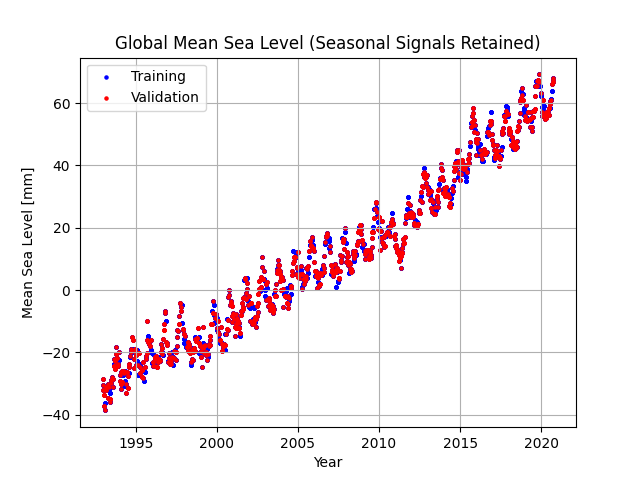
\includegraphics[width=\columnwidth]{figures/dataset.png}
	\label{fig:part_a}
\end{figure}

It can be seen there is a clear linear trend between year and mean sea level. The dataset was then partitioned into an 80/20 split of training and validation data. Applying linear regression to the (normalized) training data learned a line with an $b=0.9758$ and $w=0.9758$.

\LST{part\_a}

\begin{figure}[htpb]
	\centering
	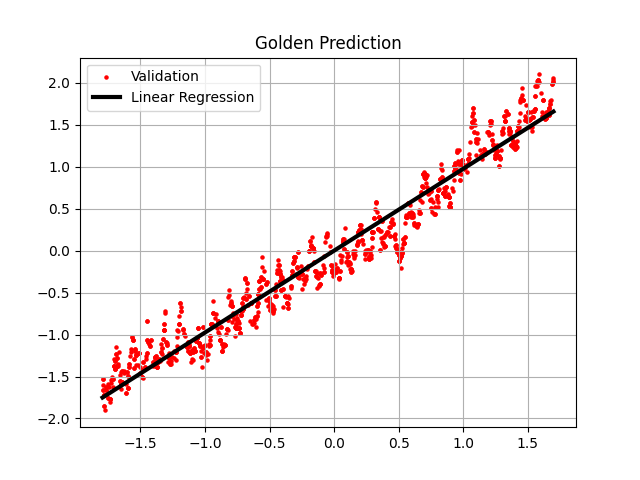
\includegraphics[width=\columnwidth]{figures/linear_regression.png}
	\label{fig:part_a}
\end{figure}

The regression line was found to have a MSE of $0.0489$
\newpage
\section{Part B}
\label{sec:sec_b}
A loss surface was created by computing the MSE for a grid of $10,000$ \textit{b} and \textit{w} pairs. Both variables were varied by $\pm3$ from the golden value found in Section~\ref{sec:sec_a}.

\begin{figure}[htpb]
	\centering
	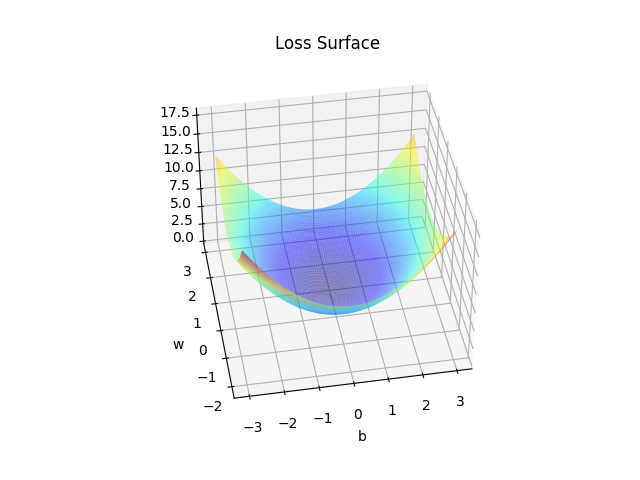
\includegraphics[width=\columnwidth]{figures/loss_surface.png}
	\label{fig:loss_surface}
\end{figure}

The above surface was generated using the following code.
\LST{part\_b}
\newpage
\section{Part C}
\label{sec:sec_c}

Next, because we are using linear regression the dataset must be made linear. In order to do so, the natural log was taken of \textit{I}$_{d}$. Linear regression was than ran by manually computing the gradients as shown in the below code. Training lasted for $500$ epochs and has a learning rate of $0.01$. MSE was used to compute the loss and the loss curve is shown in Figure~\ref{fig:loss}. After training the final value of \textit{b} and \textit{w} were found to be $-15.2738$ and $15.5091$ respectively when unnormalized. The training loss for the final epoch was $0.001532$

\LST{part\_c}

\begin{figure}[!htpb]
	\centering
	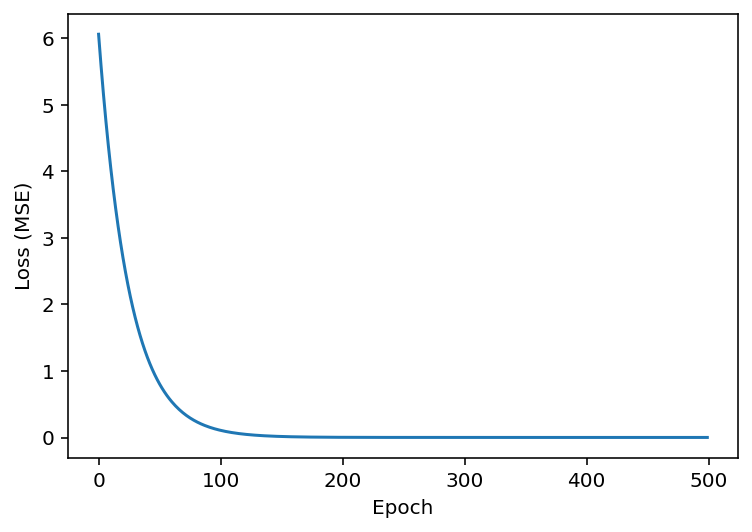
\includegraphics{figures/loss.png}
	\caption{Training Loss Curve}
	\label{fig:loss}
\end{figure}
\newpage
\section{Part D/E}
\label{sec:sec_de}

Using the learned parameters from Section~\ref{sec:sec_c} the current values in the validation set. The learned regression line is shown in Figure~\ref{fig:learn}. And the validation loss was computed to be $0.001394$ which is reasonably inline with the training loss. It being lower than the training loss can be attributed to the small dataset size and only have 10 validation points.  

\LST{part\_d}

\begin{figure}[!htpb]
	\centering
	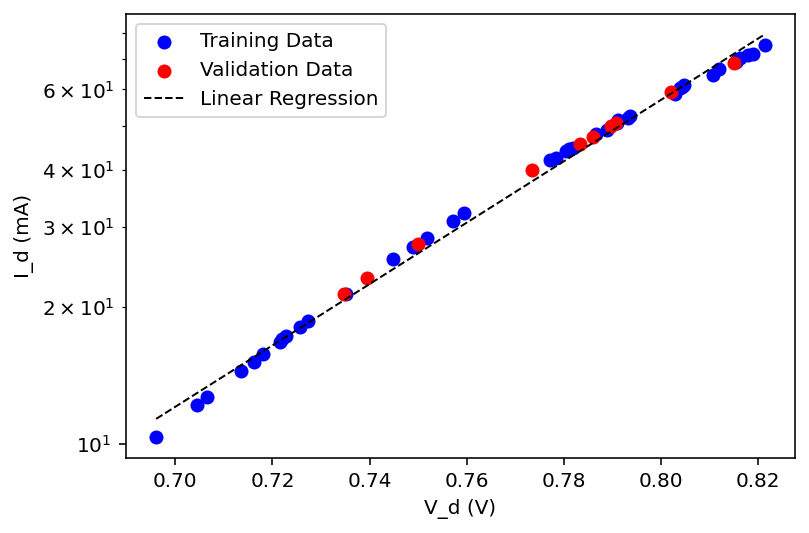
\includegraphics{figures/fit.png}
	\caption{Regression Line}
	\label{fig:fit}
\end{figure}

\newpage
\section{Part F}
\label{sec:sec_f}

In this experiment we sweep two different optimizers (\textbf{Adam} and \textbf{SGD}) across different number of training epochs. Figure~\ref{fig:f} compares the final training loss after $X$ epochs and the training time. For this experiment training was ran entirely on the CPU.

\LST{part\_f}

It can be seen that with a large number of Epochs the \textit{Adam} optimizer does eventually converge towards the same values as the \textit{SGD} optimizer. And the ADAM runtime is slightly slower.

\begin{figure}[htpb]
	\centering
	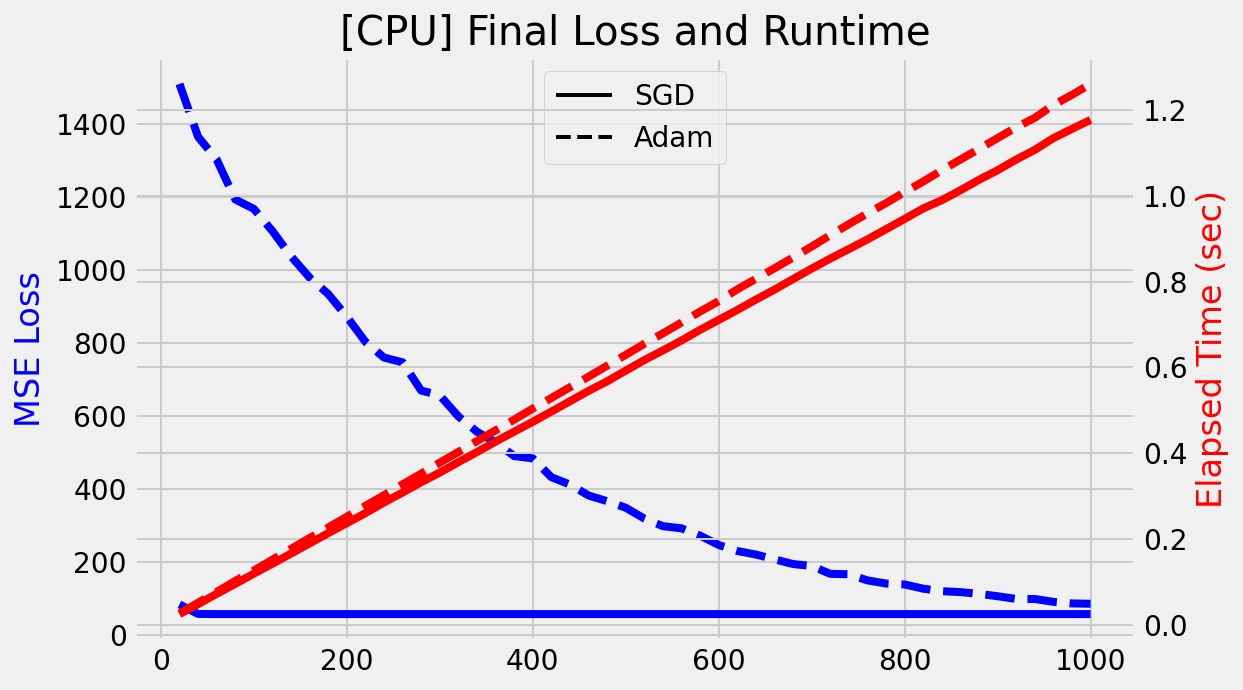
\includegraphics[width=\columnwidth]{figures/cpu_timing.png}
	\caption{CPU Final Training loss and Runtime vs Epochs}
	\label{fig:f}
\end{figure}




\end{document}

